\documentclass[a4paper, 10pt]{article}
\usepackage{fullpage} % changes the margin
\usepackage[english]{babel}
\usepackage[utf8]{inputenc}
\usepackage{hyperref}
\usepackage{xcolor}
\usepackage{graphicx}
\usepackage{array}
\usepackage{float}
\usepackage{longtable}
\usepackage[bottom]{footmisc}
\usepackage{cite}
\usepackage{parskip}
\usepackage{subcaption}
\usepackage{amssymb}
\usepackage{amsmath}
\usepackage{listings}

\hypersetup{
	colorlinks=true,       % false: boxed links; true: colored links
	linkcolor=blue,        % color of internal links
	citecolor=blue,        % color of links to bibliography
	filecolor=magenta,     % color of file links
	urlcolor=blue
}

%\setlength{\parindent}{0cm}
\newcommand{\code}[1]{\texttt{#1}}
\renewcommand{\arraystretch}{1.4}

\graphicspath{{../plots/}}

\begin{document}

\noindent
\begin{flushright}
    \large\textbf{Miguel Alcón Doganoc} \\
    Advanced Data Structures \\
	%\today
	June 21, 2019
\end{flushright}

\noindent
{\huge{\textbf{Exact String Matching Algorithms}}}

\section*{Introduction}
This document is related with the first work proposed at the Bioinformatic lectures. The purpose of this work is to check if the theory explained in class, about the search algorithms for only one pattern, is still true. As it is said in the statement, we have to compare the performance of 4 algorithms: \textit{Brute Force} (BF), \textit{Horspool} (H), \textit{Backward Nondeterministic Dawg Matching} (BNDM) and \textit{Backward Oracle Matching} (BOM). The comparison is made over a DNA alphabet file of at least 2GB, with random patterns of length $k > 0$.

\section*{Experiment}
First, I downloaded the codes of the algorithms from \cite{link} and the 2.25GB string from \cite{data}. Then, I had to modify each of the codes to let them read an external file and accept several parameters. These parameters are the DNA alphabet file and $n$ pairs composed by the size of a pattern and the pattern itself. As an example of how to call one of the algorithms:
\[
	\text{\$ ./algorithm file\_path size$_1$ pattern$_1$ size$_2$ pattern$_2$ ... size$_n$ pattern$_n$}
\]
Moreover, I created a \textit{Python} script to generate a random pattern of length $k$ (input). Finally, I created a \textit{Bash} script that is in charge of generating a string with all the parameters, and then to call each of the algorithms with it. I executed it with $n = 100$, with the size of the patterns from 10 to 1000 with steps of 10, but once $k > 10$ it does not find anything. So I executed it again with $n = 100$, but with the size of the patterns from 1 to 20.

\section*{Results}
As you can see in figure \ref{fig:time} and \ref{fig:best}, the best algorithm when searching small patterns ($k \leq 5$) is H, and BNDM is the best when searching big ones ($k > 5$). In figure \ref{fig:found} we can check that all the algorithms find the same number of patterns. Because the difference between the found patterns with $k = 1$ and $k = 15$ is huge (429877019 v.s. 1), in the figure you cannot see clear the number of patterns found. I put them in table \ref{tab}. With this, we can conclude that the theory explained in class is true.

\begin{figure}[htbp]
	\centering
	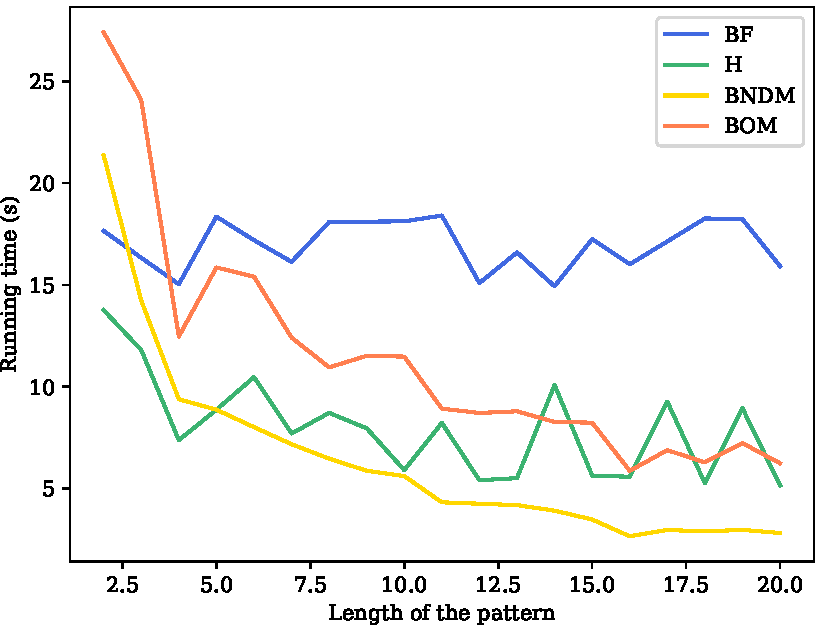
\includegraphics[width=0.75\linewidth]{time.pdf}
	\caption{Running time of each algorithm}
	\label{fig:time}
\end{figure}

\begin{figure}[htbp]
	\centering
	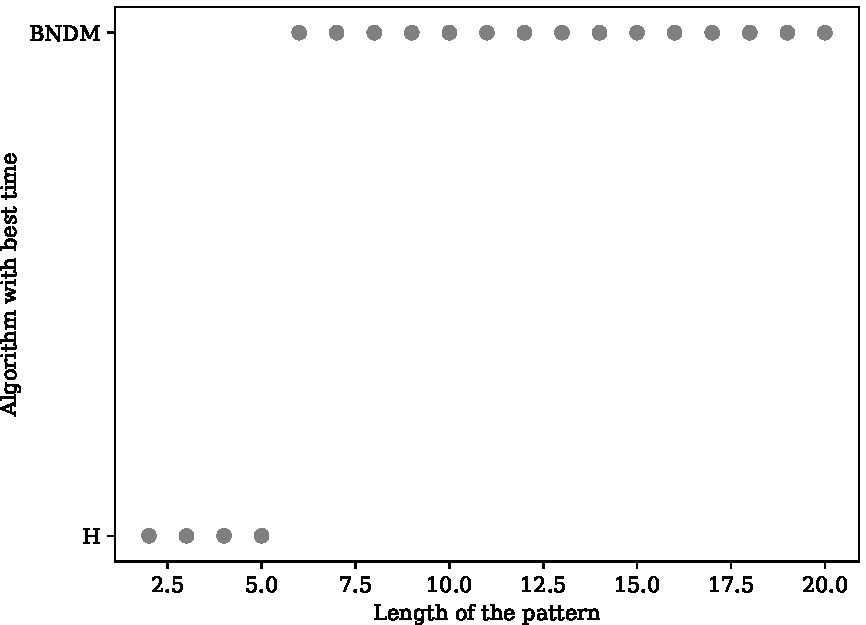
\includegraphics[width=0.75\linewidth]{best.pdf}
	\caption{Best algorithms}
	\label{fig:best}
\end{figure}

\begin{figure}[htbp]
	\centering
	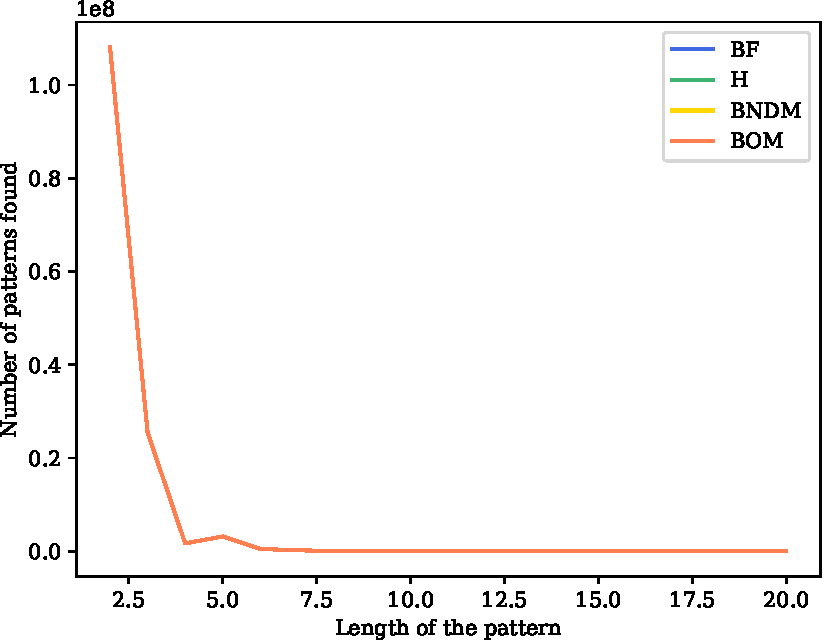
\includegraphics[width=0.75\linewidth]{found.pdf}
	\caption{Number of patterns found}
	\label{fig:found}
\end{figure}

\begin{table}
	\centering
	\begin{tabular}{c c}
		Length of the pattern & Number of patterns found \\ \hline
		1 & 429877019 \\
		2 & 108081606 \\
		3 & 25462401 \\
		4 & 1697740 \\
		5 & 3180369 \\
		6 & 499409 \\
		7 & 211306 \\
		8 & 58644 \\
		9 & 9120 \\
		10 & 3056 \\
		11 & 100 \\
		12 & 263 \\
		13 & 35 \\
		14 & 3 \\
		15 & 1 \\
		16 & 0 \\
		17 & 0 \\
		18 & 0 \\
		19 & 0 \\
		20 & 0 \\
	\end{tabular}
	\caption{Number of patterns found depending on the length of the pattern}
	\label{tab}
\end{table}

\bibliographystyle{unsrt}
\bibliography{cite}


\end{document}